% Options for packages loaded elsewhere
\PassOptionsToPackage{unicode}{hyperref}
\PassOptionsToPackage{hyphens}{url}
%
\documentclass[
]{article}
\usepackage{amsmath,amssymb}
\usepackage{lmodern}
\usepackage{iftex}
\ifPDFTeX
  \usepackage[T1]{fontenc}
  \usepackage[utf8]{inputenc}
  \usepackage{textcomp} % provide euro and other symbols
\else % if luatex or xetex
  \usepackage{unicode-math}
  \defaultfontfeatures{Scale=MatchLowercase}
  \defaultfontfeatures[\rmfamily]{Ligatures=TeX,Scale=1}
\fi
% Use upquote if available, for straight quotes in verbatim environments
\IfFileExists{upquote.sty}{\usepackage{upquote}}{}
\IfFileExists{microtype.sty}{% use microtype if available
  \usepackage[]{microtype}
  \UseMicrotypeSet[protrusion]{basicmath} % disable protrusion for tt fonts
}{}
\makeatletter
\@ifundefined{KOMAClassName}{% if non-KOMA class
  \IfFileExists{parskip.sty}{%
    \usepackage{parskip}
  }{% else
    \setlength{\parindent}{0pt}
    \setlength{\parskip}{6pt plus 2pt minus 1pt}}
}{% if KOMA class
  \KOMAoptions{parskip=half}}
\makeatother
\usepackage{xcolor}
\IfFileExists{xurl.sty}{\usepackage{xurl}}{} % add URL line breaks if available
\IfFileExists{bookmark.sty}{\usepackage{bookmark}}{\usepackage{hyperref}}
\hypersetup{
  hidelinks,
  pdfcreator={LaTeX via pandoc}}
\urlstyle{same} % disable monospaced font for URLs
\usepackage{color}
\usepackage{fancyvrb}
\newcommand{\VerbBar}{|}
\newcommand{\VERB}{\Verb[commandchars=\\\{\}]}
\DefineVerbatimEnvironment{Highlighting}{Verbatim}{commandchars=\\\{\}}
% Add ',fontsize=\small' for more characters per line
\usepackage{framed}
\definecolor{shadecolor}{RGB}{248,248,248}
\newenvironment{Shaded}{\begin{snugshade}}{\end{snugshade}}
\newcommand{\AlertTok}[1]{\textcolor[rgb]{0.94,0.16,0.16}{#1}}
\newcommand{\AnnotationTok}[1]{\textcolor[rgb]{0.56,0.35,0.01}{\textbf{\textit{#1}}}}
\newcommand{\AttributeTok}[1]{\textcolor[rgb]{0.77,0.63,0.00}{#1}}
\newcommand{\BaseNTok}[1]{\textcolor[rgb]{0.00,0.00,0.81}{#1}}
\newcommand{\BuiltInTok}[1]{#1}
\newcommand{\CharTok}[1]{\textcolor[rgb]{0.31,0.60,0.02}{#1}}
\newcommand{\CommentTok}[1]{\textcolor[rgb]{0.56,0.35,0.01}{\textit{#1}}}
\newcommand{\CommentVarTok}[1]{\textcolor[rgb]{0.56,0.35,0.01}{\textbf{\textit{#1}}}}
\newcommand{\ConstantTok}[1]{\textcolor[rgb]{0.00,0.00,0.00}{#1}}
\newcommand{\ControlFlowTok}[1]{\textcolor[rgb]{0.13,0.29,0.53}{\textbf{#1}}}
\newcommand{\DataTypeTok}[1]{\textcolor[rgb]{0.13,0.29,0.53}{#1}}
\newcommand{\DecValTok}[1]{\textcolor[rgb]{0.00,0.00,0.81}{#1}}
\newcommand{\DocumentationTok}[1]{\textcolor[rgb]{0.56,0.35,0.01}{\textbf{\textit{#1}}}}
\newcommand{\ErrorTok}[1]{\textcolor[rgb]{0.64,0.00,0.00}{\textbf{#1}}}
\newcommand{\ExtensionTok}[1]{#1}
\newcommand{\FloatTok}[1]{\textcolor[rgb]{0.00,0.00,0.81}{#1}}
\newcommand{\FunctionTok}[1]{\textcolor[rgb]{0.00,0.00,0.00}{#1}}
\newcommand{\ImportTok}[1]{#1}
\newcommand{\InformationTok}[1]{\textcolor[rgb]{0.56,0.35,0.01}{\textbf{\textit{#1}}}}
\newcommand{\KeywordTok}[1]{\textcolor[rgb]{0.13,0.29,0.53}{\textbf{#1}}}
\newcommand{\NormalTok}[1]{#1}
\newcommand{\OperatorTok}[1]{\textcolor[rgb]{0.81,0.36,0.00}{\textbf{#1}}}
\newcommand{\OtherTok}[1]{\textcolor[rgb]{0.56,0.35,0.01}{#1}}
\newcommand{\PreprocessorTok}[1]{\textcolor[rgb]{0.56,0.35,0.01}{\textit{#1}}}
\newcommand{\RegionMarkerTok}[1]{#1}
\newcommand{\SpecialCharTok}[1]{\textcolor[rgb]{0.00,0.00,0.00}{#1}}
\newcommand{\SpecialStringTok}[1]{\textcolor[rgb]{0.31,0.60,0.02}{#1}}
\newcommand{\StringTok}[1]{\textcolor[rgb]{0.31,0.60,0.02}{#1}}
\newcommand{\VariableTok}[1]{\textcolor[rgb]{0.00,0.00,0.00}{#1}}
\newcommand{\VerbatimStringTok}[1]{\textcolor[rgb]{0.31,0.60,0.02}{#1}}
\newcommand{\WarningTok}[1]{\textcolor[rgb]{0.56,0.35,0.01}{\textbf{\textit{#1}}}}
\usepackage{longtable,booktabs,array}
\usepackage{calc} % for calculating minipage widths
% Correct order of tables after \paragraph or \subparagraph
\usepackage{etoolbox}
\makeatletter
\patchcmd\longtable{\par}{\if@noskipsec\mbox{}\fi\par}{}{}
\makeatother
% Allow footnotes in longtable head/foot
\IfFileExists{footnotehyper.sty}{\usepackage{footnotehyper}}{\usepackage{footnote}}
\makesavenoteenv{longtable}
\usepackage{graphicx}
\makeatletter
\def\maxwidth{\ifdim\Gin@nat@width>\linewidth\linewidth\else\Gin@nat@width\fi}
\def\maxheight{\ifdim\Gin@nat@height>\textheight\textheight\else\Gin@nat@height\fi}
\makeatother
% Scale images if necessary, so that they will not overflow the page
% margins by default, and it is still possible to overwrite the defaults
% using explicit options in \includegraphics[width, height, ...]{}
\setkeys{Gin}{width=\maxwidth,height=\maxheight,keepaspectratio}
% Set default figure placement to htbp
\makeatletter
\def\fps@figure{htbp}
\makeatother
\setlength{\emergencystretch}{3em} % prevent overfull lines
\providecommand{\tightlist}{%
  \setlength{\itemsep}{0pt}\setlength{\parskip}{0pt}}
\setcounter{secnumdepth}{5}
\usepackage{booktabs}
\ifLuaTeX
  \usepackage{selnolig}  % disable illegal ligatures
\fi
\usepackage[]{natbib}
\bibliographystyle{plainnat}

\author{}
\date{\vspace{-2.5em}}

\begin{document}

{
\setcounter{tocdepth}{2}
\tableofcontents
}
\begin{longtable}[]{@{}
  >{\raggedright\arraybackslash}p{(\columnwidth - 0\tabcolsep) * \real{0.0694}}@{}}
\toprule
\endhead
title: ``Biometry for Clinical Research''
author: ``Kishore Puthezhath''
date: ``2022-01-12''
site: bookdown::bookdown\_site
documentclass: book
bibliography: {[}book.bib, packages.bib{]}
\# url: your book url like \url{https://bookdown.org/yihui/bookdown}
\# cover-image: path to the social sharing image like images/cover.jpg
description: \textbar{} \\
biblio-style: apalike
csl: chicago-fullnote-bibliography.csl \\
\bottomrule
\end{longtable}

\hypertarget{about}{%
\section{About}\label{about}}

``Scientific etiquette demands that a field be defined before its study is begun''-R R Sokal. \emph{Bios} means ``life'' and \emph{metron} means ``measure''.

\hypertarget{r-basics}{%
\section{r Basics}\label{r-basics}}

\begin{Shaded}
\begin{Highlighting}[]
\CommentTok{\# find out the working directory}
\FunctionTok{getwd}\NormalTok{()}
\CommentTok{\#\textgreater{} [1] "/Users/drkmenon/Sync/books/biometry"}
\CommentTok{\# setwd in R}

\FunctionTok{setwd}\NormalTok{(}\StringTok{"/Users/drkmenon/"}\NormalTok{)}

\FunctionTok{getwd}\NormalTok{()}
\CommentTok{\#\textgreater{} [1] "/Users/drkmenon"}

\DocumentationTok{\#\# change back}
\end{Highlighting}
\end{Shaded}

\begin{Shaded}
\begin{Highlighting}[]
\FunctionTok{setwd}\NormalTok{(}\StringTok{"/Users/drkmenon/Sync/books/biometry"}\NormalTok{)}
\FunctionTok{getwd}\NormalTok{()}
\CommentTok{\#\textgreater{} [1] "/Users/drkmenon/Sync/books/biometry"}

\CommentTok{\# tab key will popout a list of things we may be looking for after entering }
\CommentTok{\# first 1{-}2 alphabets}

\CommentTok{\# save this as a project}

\CommentTok{\# myrstats\textless{}{-}save.image("myrstats.rData")}

\CommentTok{\# Essential packages}
\end{Highlighting}
\end{Shaded}

\begin{Shaded}
\begin{Highlighting}[]
\FunctionTok{library}\NormalTok{(knitr)}
\FunctionTok{library}\NormalTok{(tidyverse)}
\CommentTok{\#\textgreater{} {-}{-} Attaching packages {-}{-}{-}{-}{-}{-}{-}{-}{-}{-}{-}{-}{-}{-}{-}{-}{-}{-}{-} tidyverse 1.3.1 {-}{-}}
\CommentTok{\#\textgreater{} v ggplot2 3.3.5     v purrr   0.3.4}
\CommentTok{\#\textgreater{} v tibble  3.1.5     v dplyr   1.0.7}
\CommentTok{\#\textgreater{} v tidyr   1.1.4     v stringr 1.4.0}
\CommentTok{\#\textgreater{} v readr   2.0.2     v forcats 0.5.1}
\CommentTok{\#\textgreater{} {-}{-} Conflicts {-}{-}{-}{-}{-}{-}{-}{-}{-}{-}{-}{-}{-}{-}{-}{-}{-}{-}{-}{-}{-}{-} tidyverse\_conflicts() {-}{-}}
\CommentTok{\#\textgreater{} x dplyr::filter() masks stats::filter()}
\CommentTok{\#\textgreater{} x dplyr::lag()    masks stats::lag()}
\FunctionTok{library}\NormalTok{(epiR)}
\CommentTok{\#\textgreater{} Loading required package: survival}
\CommentTok{\#\textgreater{} Package epiR 2.0.39 is loaded}
\CommentTok{\#\textgreater{} Type help(epi.about) for summary information}
\CommentTok{\#\textgreater{} Type browseVignettes(package = \textquotesingle{}epiR\textquotesingle{}) to learn how to use epiR for applied epidemiological analyses}
\CommentTok{\#\textgreater{} }
\FunctionTok{library}\NormalTok{(epiDisplay)}
\CommentTok{\#\textgreater{} Loading required package: foreign}
\CommentTok{\#\textgreater{} Loading required package: MASS}
\CommentTok{\#\textgreater{} }
\CommentTok{\#\textgreater{} Attaching package: \textquotesingle{}MASS\textquotesingle{}}
\CommentTok{\#\textgreater{} The following object is masked from \textquotesingle{}package:dplyr\textquotesingle{}:}
\CommentTok{\#\textgreater{} }
\CommentTok{\#\textgreater{}     select}
\CommentTok{\#\textgreater{} Loading required package: nnet}
\CommentTok{\#\textgreater{} }
\CommentTok{\#\textgreater{} Attaching package: \textquotesingle{}epiDisplay\textquotesingle{}}
\CommentTok{\#\textgreater{} The following object is masked from \textquotesingle{}package:ggplot2\textquotesingle{}:}
\CommentTok{\#\textgreater{} }
\CommentTok{\#\textgreater{}     alpha}
\FunctionTok{library}\NormalTok{(survival)}
\FunctionTok{library}\NormalTok{(survminer)}
\CommentTok{\#\textgreater{} Loading required package: ggpubr}
\FunctionTok{library}\NormalTok{(randomizeR)}
\CommentTok{\#\textgreater{} Loading required package: plotrix}
\end{Highlighting}
\end{Shaded}

\begin{Shaded}
\begin{Highlighting}[]
\NormalTok{x}\OtherTok{\textless{}{-}} \DecValTok{2}
\NormalTok{x}
\CommentTok{\#\textgreater{} [1] 2}
\end{Highlighting}
\end{Shaded}

x is an object containing variable 2

\begin{Shaded}
\begin{Highlighting}[]
\NormalTok{y}\OtherTok{\textless{}{-}}\StringTok{"male"}
\NormalTok{y}
\CommentTok{\#\textgreater{} [1] "male"}
\end{Highlighting}
\end{Shaded}

y is an object containing variable ``male''
x is numeric/integer and ``male'' is factor/character
factors can be grouped for analysis, characters cannot be

\begin{Shaded}
\begin{Highlighting}[]
\FunctionTok{class}\NormalTok{(x)}
\CommentTok{\#\textgreater{} [1] "numeric"}
\FunctionTok{class}\NormalTok{(y)}
\CommentTok{\#\textgreater{} [1] "character"}
\end{Highlighting}
\end{Shaded}

Convert character to factor

\begin{Shaded}
\begin{Highlighting}[]
\NormalTok{z}\OtherTok{=} \FunctionTok{as.factor}\NormalTok{(y)}
\FunctionTok{class}\NormalTok{(z)}
\CommentTok{\#\textgreater{} [1] "factor"}
\end{Highlighting}
\end{Shaded}

concatenation: it is a string of interconnected things

\begin{Shaded}
\begin{Highlighting}[]
\NormalTok{x1}\OtherTok{\textless{}{-}} \FunctionTok{c}\NormalTok{(}\DecValTok{1}\NormalTok{,}\DecValTok{2}\NormalTok{,}\DecValTok{3}\NormalTok{,}\DecValTok{4}\NormalTok{,}\DecValTok{5}\NormalTok{)}
\NormalTok{x1}
\CommentTok{\#\textgreater{} [1] 1 2 3 4 5}
\end{Highlighting}
\end{Shaded}

different methods of producing concatenated vectors

\begin{Shaded}
\begin{Highlighting}[]
\NormalTok{x1}\OtherTok{\textless{}{-}}\FunctionTok{c}\NormalTok{(}\DecValTok{1}\SpecialCharTok{:}\DecValTok{5}\NormalTok{)}
\NormalTok{x1}\OtherTok{\textless{}{-}}\FunctionTok{seq}\NormalTok{(}\AttributeTok{from=}\DecValTok{1}\NormalTok{, }\AttributeTok{to=}\DecValTok{5}\NormalTok{, }\AttributeTok{by=}\DecValTok{1}\NormalTok{)}
\NormalTok{x1}
\CommentTok{\#\textgreater{} [1] 1 2 3 4 5}
\end{Highlighting}
\end{Shaded}

we can also create repeated sequence in R

\begin{Shaded}
\begin{Highlighting}[]
\NormalTok{x2}\OtherTok{\textless{}{-}}\FunctionTok{rep}\NormalTok{(}\DecValTok{1}\NormalTok{, }\AttributeTok{times=}\DecValTok{5}\NormalTok{)}
\NormalTok{x2}
\CommentTok{\#\textgreater{} [1] 1 1 1 1 1}

\NormalTok{x3}\OtherTok{\textless{}{-}}\FunctionTok{rep}\NormalTok{(}\FunctionTok{seq}\NormalTok{(}\AttributeTok{from=}\DecValTok{2}\NormalTok{, }\AttributeTok{to=}\DecValTok{6}\NormalTok{, }\AttributeTok{by=}\FloatTok{0.05}\NormalTok{), }\AttributeTok{times=}\DecValTok{5}\NormalTok{)}
\NormalTok{x3}
\CommentTok{\#\textgreater{}   [1] 2.00 2.05 2.10 2.15 2.20 2.25 2.30 2.35 2.40 2.45 2.50}
\CommentTok{\#\textgreater{}  [12] 2.55 2.60 2.65 2.70 2.75 2.80 2.85 2.90 2.95 3.00 3.05}
\CommentTok{\#\textgreater{}  [23] 3.10 3.15 3.20 3.25 3.30 3.35 3.40 3.45 3.50 3.55 3.60}
\CommentTok{\#\textgreater{}  [34] 3.65 3.70 3.75 3.80 3.85 3.90 3.95 4.00 4.05 4.10 4.15}
\CommentTok{\#\textgreater{}  [45] 4.20 4.25 4.30 4.35 4.40 4.45 4.50 4.55 4.60 4.65 4.70}
\CommentTok{\#\textgreater{}  [56] 4.75 4.80 4.85 4.90 4.95 5.00 5.05 5.10 5.15 5.20 5.25}
\CommentTok{\#\textgreater{}  [67] 5.30 5.35 5.40 5.45 5.50 5.55 5.60 5.65 5.70 5.75 5.80}
\CommentTok{\#\textgreater{}  [78] 5.85 5.90 5.95 6.00 2.00 2.05 2.10 2.15 2.20 2.25 2.30}
\CommentTok{\#\textgreater{}  [89] 2.35 2.40 2.45 2.50 2.55 2.60 2.65 2.70 2.75 2.80 2.85}
\CommentTok{\#\textgreater{} [100] 2.90 2.95 3.00 3.05 3.10 3.15 3.20 3.25 3.30 3.35 3.40}
\CommentTok{\#\textgreater{} [111] 3.45 3.50 3.55 3.60 3.65 3.70 3.75 3.80 3.85 3.90 3.95}
\CommentTok{\#\textgreater{} [122] 4.00 4.05 4.10 4.15 4.20 4.25 4.30 4.35 4.40 4.45 4.50}
\CommentTok{\#\textgreater{} [133] 4.55 4.60 4.65 4.70 4.75 4.80 4.85 4.90 4.95 5.00 5.05}
\CommentTok{\#\textgreater{} [144] 5.10 5.15 5.20 5.25 5.30 5.35 5.40 5.45 5.50 5.55 5.60}
\CommentTok{\#\textgreater{} [155] 5.65 5.70 5.75 5.80 5.85 5.90 5.95 6.00 2.00 2.05 2.10}
\CommentTok{\#\textgreater{} [166] 2.15 2.20 2.25 2.30 2.35 2.40 2.45 2.50 2.55 2.60 2.65}
\CommentTok{\#\textgreater{} [177] 2.70 2.75 2.80 2.85 2.90 2.95 3.00 3.05 3.10 3.15 3.20}
\CommentTok{\#\textgreater{} [188] 3.25 3.30 3.35 3.40 3.45 3.50 3.55 3.60 3.65 3.70 3.75}
\CommentTok{\#\textgreater{} [199] 3.80 3.85 3.90 3.95 4.00 4.05 4.10 4.15 4.20 4.25 4.30}
\CommentTok{\#\textgreater{} [210] 4.35 4.40 4.45 4.50 4.55 4.60 4.65 4.70 4.75 4.80 4.85}
\CommentTok{\#\textgreater{} [221] 4.90 4.95 5.00 5.05 5.10 5.15 5.20 5.25 5.30 5.35 5.40}
\CommentTok{\#\textgreater{} [232] 5.45 5.50 5.55 5.60 5.65 5.70 5.75 5.80 5.85 5.90 5.95}
\CommentTok{\#\textgreater{} [243] 6.00 2.00 2.05 2.10 2.15 2.20 2.25 2.30 2.35 2.40 2.45}
\CommentTok{\#\textgreater{} [254] 2.50 2.55 2.60 2.65 2.70 2.75 2.80 2.85 2.90 2.95 3.00}
\CommentTok{\#\textgreater{} [265] 3.05 3.10 3.15 3.20 3.25 3.30 3.35 3.40 3.45 3.50 3.55}
\CommentTok{\#\textgreater{} [276] 3.60 3.65 3.70 3.75 3.80 3.85 3.90 3.95 4.00 4.05 4.10}
\CommentTok{\#\textgreater{} [287] 4.15 4.20 4.25 4.30 4.35 4.40 4.45 4.50 4.55 4.60 4.65}
\CommentTok{\#\textgreater{} [298] 4.70 4.75 4.80 4.85 4.90 4.95 5.00 5.05 5.10 5.15 5.20}
\CommentTok{\#\textgreater{} [309] 5.25 5.30 5.35 5.40 5.45 5.50 5.55 5.60 5.65 5.70 5.75}
\CommentTok{\#\textgreater{} [320] 5.80 5.85 5.90 5.95 6.00 2.00 2.05 2.10 2.15 2.20 2.25}
\CommentTok{\#\textgreater{} [331] 2.30 2.35 2.40 2.45 2.50 2.55 2.60 2.65 2.70 2.75 2.80}
\CommentTok{\#\textgreater{} [342] 2.85 2.90 2.95 3.00 3.05 3.10 3.15 3.20 3.25 3.30 3.35}
\CommentTok{\#\textgreater{} [353] 3.40 3.45 3.50 3.55 3.60 3.65 3.70 3.75 3.80 3.85 3.90}
\CommentTok{\#\textgreater{} [364] 3.95 4.00 4.05 4.10 4.15 4.20 4.25 4.30 4.35 4.40 4.45}
\CommentTok{\#\textgreater{} [375] 4.50 4.55 4.60 4.65 4.70 4.75 4.80 4.85 4.90 4.95 5.00}
\CommentTok{\#\textgreater{} [386] 5.05 5.10 5.15 5.20 5.25 5.30 5.35 5.40 5.45 5.50 5.55}
\CommentTok{\#\textgreater{} [397] 5.60 5.65 5.70 5.75 5.80 5.85 5.90 5.95 6.00}
\end{Highlighting}
\end{Shaded}

extracting elements from concatenated string

\begin{Shaded}
\begin{Highlighting}[]
\NormalTok{x1}
\CommentTok{\#\textgreater{} [1] 1 2 3 4 5}
\NormalTok{x1[}\DecValTok{3}\NormalTok{]}
\CommentTok{\#\textgreater{} [1] 3}
\NormalTok{x1[}\DecValTok{1}\SpecialCharTok{:}\DecValTok{3}\NormalTok{]}
\CommentTok{\#\textgreater{} [1] 1 2 3}
\NormalTok{x1[}\FunctionTok{c}\NormalTok{(}\DecValTok{2}\NormalTok{,}\DecValTok{4}\NormalTok{)]}
\CommentTok{\#\textgreater{} [1] 2 4}
\NormalTok{x1[}\SpecialCharTok{{-}}\DecValTok{1}\NormalTok{]}
\CommentTok{\#\textgreater{} [1] 2 3 4 5}
\end{Highlighting}
\end{Shaded}

Matrix of elements
Vector is a list of numbers/characters
Matrix is an array of numbers/characters in raws and columns

\begin{Shaded}
\begin{Highlighting}[]
\NormalTok{m1}\OtherTok{\textless{}{-}}\FunctionTok{matrix}\NormalTok{(}\FunctionTok{c}\NormalTok{(}\DecValTok{1}\SpecialCharTok{:}\DecValTok{20}\NormalTok{),}\AttributeTok{nrow=}\DecValTok{5}\NormalTok{, }\AttributeTok{byrow=}\NormalTok{T)}
\NormalTok{m1}
\CommentTok{\#\textgreater{}      [,1] [,2] [,3] [,4]}
\CommentTok{\#\textgreater{} [1,]    1    2    3    4}
\CommentTok{\#\textgreater{} [2,]    5    6    7    8}
\CommentTok{\#\textgreater{} [3,]    9   10   11   12}
\CommentTok{\#\textgreater{} [4,]   13   14   15   16}
\CommentTok{\#\textgreater{} [5,]   17   18   19   20}
\end{Highlighting}
\end{Shaded}

similar to vectors, matrix can be subsetted

\begin{Shaded}
\begin{Highlighting}[]
\NormalTok{m1[}\FunctionTok{c}\NormalTok{(}\DecValTok{2}\NormalTok{,}\DecValTok{3}\NormalTok{), }\DecValTok{2}\NormalTok{]}
\CommentTok{\#\textgreater{} [1]  6 10}
\end{Highlighting}
\end{Shaded}

data\_frame is a type of matrix
we can create data\_frame in R or we can import

Creating data\_frame
first we have to create concatenated strings of variable
name\textless-c(letters{[}1:10{]})
age\textless-seq(from=63, to=82, by=2)
type\_surg\textless- c(0,1,0,0,1,1,1,0,0,0)

\hypertarget{r-recognizes-this-as-a-number-series-we-have-to-covert-this-to-factor}{%
\section{R recognizes this as a number series, we have to covert this to factor}\label{r-recognizes-this-as-a-number-series-we-have-to-covert-this-to-factor}}

type\_surg\textless-as.factor(type\_surg)

pri\_event\textless-c(0,0,0,0,0,1,1,0,0,1)
pri\_event\textless-as.factor(pri\_event)
time\textless-c(24,24,24,24,24,3,2,24,24,7)
test\_data\textless- data.frame(name,age,type\_surg,pri\_event,time)
test\_data

\hypertarget{subsetting-can-be-done.-important-to-remember-to-specify-the-column-as-blank}{%
\section{subsetting can be done. important to remember to specify the column as blank}\label{subsetting-can-be-done.-important-to-remember-to-specify-the-column-as-blank}}

\hypertarget{after-a-coma}{%
\section{after a coma}\label{after-a-coma}}

ageo70\textless-test\_data{[}age\textgreater70,{]}
ageo70

\begin{verbatim}

<!--chapter:end:1.1-rbasics.Rmd-->

# Data handling


```r
# create data_frame

# first we have to create concatenated strings of variable
name<-c(letters[1:10])
age<-seq(from=63, to=82, by=2)
type_surg<- c(0,1,0,0,1,1,1,0,0,0)

# R recognizes this as a number series, we have to covert this to factor
type_surg<-as.factor(type_surg)

pri_event<-c(0,0,0,0,0,1,1,0,0,1)
pri_event<-as.factor(pri_event)
time<-c(24,24,24,24,24,3,2,24,24,7)
test_data<- data.frame(name,age,type_surg,pri_event,time)
test_data
#>    name age type_surg pri_event time
#> 1     a  63         0         0   24
#> 2     b  65         1         0   24
#> 3     c  67         0         0   24
#> 4     d  69         0         0   24
#> 5     e  71         1         0   24
#> 6     f  73         1         1    3
#> 7     g  75         1         1    2
#> 8     h  77         0         0   24
#> 9     i  79         0         0   24
#> 10    j  81         0         1    7

#logic operations

# add new row to test_data2, cbind and rbind

new_data<-c("k", 63,0,0,24)
new_data
#> [1] "k"  "63" "0"  "0"  "24"

test_data2<-rbind(test_data,new_data)
test_data2
#>    name age type_surg pri_event time
#> 1     a  63         0         0   24
#> 2     b  65         1         0   24
#> 3     c  67         0         0   24
#> 4     d  69         0         0   24
#> 5     e  71         1         0   24
#> 6     f  73         1         1    3
#> 7     g  75         1         1    2
#> 8     h  77         0         0   24
#> 9     i  79         0         0   24
#> 10    j  81         0         1    7
#> 11    k  63         0         0   24

new_data2<-c(10:1)
test_data3<-cbind(test_data,new_data2)
test_data3
#>    name age type_surg pri_event time new_data2
#> 1     a  63         0         0   24        10
#> 2     b  65         1         0   24         9
#> 3     c  67         0         0   24         8
#> 4     d  69         0         0   24         7
#> 5     e  71         1         0   24         6
#> 6     f  73         1         1    3         5
#> 7     g  75         1         1    2         4
#> 8     h  77         0         0   24         3
#> 9     i  79         0         0   24         2
#> 10    j  81         0         1    7         1

# other logic operations, on the test_data in the r basics script

# is age >70?

typage<-age>70
typage[1:5]
#> [1] FALSE FALSE FALSE FALSE  TRUE

# get this answer as 0 and 1

typage2<-as.numeric(age>70)
typage2  
#>  [1] 0 0 0 0 1 1 1 1 1 1

# multiple logic operations

oldtha<-age>70 & type_surg=="1"
oldtha
#>  [1] FALSE FALSE FALSE FALSE  TRUE  TRUE  TRUE FALSE FALSE
#> [10] FALSE

# add this to our data as a new column

test_data
#>    name age type_surg pri_event time
#> 1     a  63         0         0   24
#> 2     b  65         1         0   24
#> 3     c  67         0         0   24
#> 4     d  69         0         0   24
#> 5     e  71         1         0   24
#> 6     f  73         1         1    3
#> 7     g  75         1         1    2
#> 8     h  77         0         0   24
#> 9     i  79         0         0   24
#> 10    j  81         0         1    7
test_data5<-cbind(test_data,oldtha)
test_data5
#>    name age type_surg pri_event time oldtha
#> 1     a  63         0         0   24  FALSE
#> 2     b  65         1         0   24  FALSE
#> 3     c  67         0         0   24  FALSE
#> 4     d  69         0         0   24  FALSE
#> 5     e  71         1         0   24   TRUE
#> 6     f  73         1         1    3   TRUE
#> 7     g  75         1         1    2   TRUE
#> 8     h  77         0         0   24  FALSE
#> 9     i  79         0         0   24  FALSE
#> 10    j  81         0         1    7  FALSE

# Clearing workspace inr

rm(list=ls())

# remember how to import dataset.
# new_datax<-read.csv(file.choose(), header = T)

# create table
# table()
\end{verbatim}

\hypertarget{data-cleaning}{%
\section{Data Cleaning}\label{data-cleaning}}

Main actions are select(), filter(), group\_by(), mutate(), summarise(),full\_join(), pivot\_wide() and pivot\_long(), spread(), map(), strsplit()

\begin{Shaded}
\begin{Highlighting}[]
\FunctionTok{library}\NormalTok{(tidyverse)}
\CommentTok{\#\textgreater{} {-}{-} Attaching packages {-}{-}{-}{-}{-}{-}{-}{-}{-}{-}{-}{-}{-}{-}{-}{-}{-}{-}{-} tidyverse 1.3.1 {-}{-}}
\CommentTok{\#\textgreater{} v ggplot2 3.3.5     v purrr   0.3.4}
\CommentTok{\#\textgreater{} v tibble  3.1.5     v dplyr   1.0.7}
\CommentTok{\#\textgreater{} v tidyr   1.1.4     v stringr 1.4.0}
\CommentTok{\#\textgreater{} v readr   2.0.2     v forcats 0.5.1}
\CommentTok{\#\textgreater{} {-}{-} Conflicts {-}{-}{-}{-}{-}{-}{-}{-}{-}{-}{-}{-}{-}{-}{-}{-}{-}{-}{-}{-}{-}{-} tidyverse\_conflicts() {-}{-}}
\CommentTok{\#\textgreater{} x dplyr::filter() masks stats::filter()}
\CommentTok{\#\textgreater{} x dplyr::lag()    masks stats::lag()}
\CommentTok{\# Use read\_csv/read\_tsv insted of read.csv}
\CommentTok{\# This will create tibble insted of data frame}
\NormalTok{booking}\OtherTok{=} \FunctionTok{read\_csv}\NormalTok{(}\StringTok{\textquotesingle{}data/bookings.csv\textquotesingle{}}\NormalTok{)}
\CommentTok{\#\textgreater{} Rows: 10000 Columns: 8}
\CommentTok{\#\textgreater{} {-}{-} Column specification {-}{-}{-}{-}{-}{-}{-}{-}{-}{-}{-}{-}{-}{-}{-}{-}{-}{-}{-}{-}{-}{-}{-}{-}{-}{-}{-}{-}{-}{-}{-}{-}{-}{-}{-}{-}}
\CommentTok{\#\textgreater{} Delimiter: ","}
\CommentTok{\#\textgreater{} chr (3): booker\_id, checkin\_day, status}
\CommentTok{\#\textgreater{} dbl (4): property\_id, room\_nights, price\_per\_night, revi...}
\CommentTok{\#\textgreater{} lgl (1): for\_business}
\CommentTok{\#\textgreater{} }
\CommentTok{\#\textgreater{} i Use \textasciigrave{}spec()\textasciigrave{} to retrieve the full column specification for this data.}
\CommentTok{\#\textgreater{} i Specify the column types or set \textasciigrave{}show\_col\_types = FALSE\textasciigrave{} to quiet this message.}
\NormalTok{property}\OtherTok{=}\FunctionTok{read\_csv}\NormalTok{(}\StringTok{\textquotesingle{}data/properties.csv\textquotesingle{}}\NormalTok{)}
\CommentTok{\#\textgreater{} Rows: 4178 Columns: 5}
\CommentTok{\#\textgreater{} {-}{-} Column specification {-}{-}{-}{-}{-}{-}{-}{-}{-}{-}{-}{-}{-}{-}{-}{-}{-}{-}{-}{-}{-}{-}{-}{-}{-}{-}{-}{-}{-}{-}{-}{-}{-}{-}{-}{-}}
\CommentTok{\#\textgreater{} Delimiter: ","}
\CommentTok{\#\textgreater{} chr (3): destination, property\_type, facilities}
\CommentTok{\#\textgreater{} dbl (2): property\_id, nr\_rooms}
\CommentTok{\#\textgreater{} }
\CommentTok{\#\textgreater{} i Use \textasciigrave{}spec()\textasciigrave{} to retrieve the full column specification for this data.}
\CommentTok{\#\textgreater{} i Specify the column types or set \textasciigrave{}show\_col\_types = FALSE\textasciigrave{} to quiet this message.}

\NormalTok{booking}
\CommentTok{\#\textgreater{} \# A tibble: 10,000 x 8}
\CommentTok{\#\textgreater{}    booker\_id         property\_id room\_nights price\_per\_night}
\CommentTok{\#\textgreater{}    \textless{}chr\textgreater{}                   \textless{}dbl\textgreater{}       \textless{}dbl\textgreater{}           \textless{}dbl\textgreater{}}
\CommentTok{\#\textgreater{}  1 215934017ba98c09\textasciitilde{}        2668           4            91.5}
\CommentTok{\#\textgreater{}  2 7f590fd6d318248a\textasciitilde{}        4656           5           107. }
\CommentTok{\#\textgreater{}  3 10f0f138e8bb1015\textasciitilde{}        4563           6            87.0}
\CommentTok{\#\textgreater{}  4 7b55021a4160dde6\textasciitilde{}        4088           7            92.4}
\CommentTok{\#\textgreater{}  5 6694a79d158c7818\textasciitilde{}        2188           4           105. }
\CommentTok{\#\textgreater{}  6 d0358740d5f15e85\textasciitilde{}        4171           2           110. }
\CommentTok{\#\textgreater{}  7 944e568a0b511b91\textasciitilde{}        2907           4           116. }
\CommentTok{\#\textgreater{}  8 95476c2ef6bb9e3c\textasciitilde{}        5141           4           111. }
\CommentTok{\#\textgreater{}  9 df235631a4c281c0\textasciitilde{}        1696           1           106. }
\CommentTok{\#\textgreater{} 10 ff610140227d40d2\textasciitilde{}        1901           7            82.3}
\CommentTok{\#\textgreater{} \# ... with 9,990 more rows, and 4 more variables:}
\CommentTok{\#\textgreater{} \#   checkin\_day \textless{}chr\textgreater{}, for\_business \textless{}lgl\textgreater{}, status \textless{}chr\textgreater{},}
\CommentTok{\#\textgreater{} \#   review\_score \textless{}dbl\textgreater{}}
\NormalTok{property}
\CommentTok{\#\textgreater{} \# A tibble: 4,178 x 5}
\CommentTok{\#\textgreater{}    property\_id destination property\_type nr\_rooms facilities}
\CommentTok{\#\textgreater{}          \textless{}dbl\textgreater{} \textless{}chr\textgreater{}       \textless{}chr\textgreater{}            \textless{}dbl\textgreater{} \textless{}chr\textgreater{}     }
\CommentTok{\#\textgreater{}  1        2668 Brisbane    Hotel               32 airport s\textasciitilde{}}
\CommentTok{\#\textgreater{}  2        4656 Brisbane    Hotel               39 on{-}site r\textasciitilde{}}
\CommentTok{\#\textgreater{}  3        4563 Brisbane    Apartment            9 laundry   }
\CommentTok{\#\textgreater{}  4        4088 Brisbane    Apartment            9 kitchen,l\textasciitilde{}}
\CommentTok{\#\textgreater{}  5        2188 Brisbane    Apartment            4 parking,k\textasciitilde{}}
\CommentTok{\#\textgreater{}  6        4171 Brisbane    Apartment            5 kitchen,p\textasciitilde{}}
\CommentTok{\#\textgreater{}  7        2907 Brisbane    Hotel               22 airport s\textasciitilde{}}
\CommentTok{\#\textgreater{}  8        5141 Brisbane    Hotel               20 breakfast\textasciitilde{}}
\CommentTok{\#\textgreater{}  9        1696 Brisbane    Apartment            5 free wifi\textasciitilde{}}
\CommentTok{\#\textgreater{} 10        1901 Brisbane    Apartment           11 free wifi\textasciitilde{}}
\CommentTok{\#\textgreater{} \# ... with 4,168 more rows}

\CommentTok{\#magrittr (pipe function, keyboard short cut: command+shift+m)}
 \CommentTok{\# \%\textgreater{}\% }
\CommentTok{\# select() and filter() functions help to extract data and study it}

\NormalTok{x}\OtherTok{=}\NormalTok{booking }\SpecialCharTok{\%\textgreater{}\%} 
  \FunctionTok{select}\NormalTok{(review\_score)}
\NormalTok{x  }
\CommentTok{\#\textgreater{} \# A tibble: 10,000 x 1}
\CommentTok{\#\textgreater{}    review\_score}
\CommentTok{\#\textgreater{}           \textless{}dbl\textgreater{}}
\CommentTok{\#\textgreater{}  1        NA   }
\CommentTok{\#\textgreater{}  2        NA   }
\CommentTok{\#\textgreater{}  3         6.26}
\CommentTok{\#\textgreater{}  4         5.95}
\CommentTok{\#\textgreater{}  5         6.43}
\CommentTok{\#\textgreater{}  6        NA   }
\CommentTok{\#\textgreater{}  7         7.60}
\CommentTok{\#\textgreater{}  8        NA   }
\CommentTok{\#\textgreater{}  9         6.97}
\CommentTok{\#\textgreater{} 10        NA   }
\CommentTok{\#\textgreater{} \# ... with 9,990 more rows}

\NormalTok{y}\OtherTok{=}\NormalTok{booking }\SpecialCharTok{\%\textgreater{}\%} 
  \FunctionTok{filter}\NormalTok{(status}\SpecialCharTok{==}\StringTok{\textquotesingle{}stayed\textquotesingle{}}\SpecialCharTok{\&!}\FunctionTok{is.na}\NormalTok{(review\_score))}
\NormalTok{y}
\CommentTok{\#\textgreater{} \# A tibble: 6,183 x 8}
\CommentTok{\#\textgreater{}    booker\_id         property\_id room\_nights price\_per\_night}
\CommentTok{\#\textgreater{}    \textless{}chr\textgreater{}                   \textless{}dbl\textgreater{}       \textless{}dbl\textgreater{}           \textless{}dbl\textgreater{}}
\CommentTok{\#\textgreater{}  1 10f0f138e8bb1015\textasciitilde{}        4563           6            87.0}
\CommentTok{\#\textgreater{}  2 7b55021a4160dde6\textasciitilde{}        4088           7            92.4}
\CommentTok{\#\textgreater{}  3 6694a79d158c7818\textasciitilde{}        2188           4           105. }
\CommentTok{\#\textgreater{}  4 944e568a0b511b91\textasciitilde{}        2907           4           116. }
\CommentTok{\#\textgreater{}  5 df235631a4c281c0\textasciitilde{}        1696           1           106. }
\CommentTok{\#\textgreater{}  6 5a1442f4c7237ec5\textasciitilde{}        2307           9            84.2}
\CommentTok{\#\textgreater{}  7 39804a2e3fb2e4c6\textasciitilde{}        2907           6           112. }
\CommentTok{\#\textgreater{}  8 e150e559405ef29b\textasciitilde{}        2870           4           127. }
\CommentTok{\#\textgreater{}  9 4e9c7c21dfcf2758\textasciitilde{}        1674           5           102. }
\CommentTok{\#\textgreater{} 10 4a2b8eaf63613548\textasciitilde{}        2885           5            86.3}
\CommentTok{\#\textgreater{} \# ... with 6,173 more rows, and 4 more variables:}
\CommentTok{\#\textgreater{} \#   checkin\_day \textless{}chr\textgreater{}, for\_business \textless{}lgl\textgreater{}, status \textless{}chr\textgreater{},}
\CommentTok{\#\textgreater{} \#   review\_score \textless{}dbl\textgreater{}}
 
\NormalTok{cheap}\OtherTok{=}\NormalTok{booking }\SpecialCharTok{\%\textgreater{}\%} 
  \FunctionTok{select}\NormalTok{(review\_score,room\_nights) }\SpecialCharTok{\%\textgreater{}\%} 
  \FunctionTok{filter}\NormalTok{(booking}\SpecialCharTok{$}\NormalTok{price\_per\_night}\SpecialCharTok{\textless{}}\DecValTok{80}\NormalTok{)}
\NormalTok{cheap}
\CommentTok{\#\textgreater{} \# A tibble: 434 x 2}
\CommentTok{\#\textgreater{}    review\_score room\_nights}
\CommentTok{\#\textgreater{}           \textless{}dbl\textgreater{}       \textless{}dbl\textgreater{}}
\CommentTok{\#\textgreater{}  1         8.90           5}
\CommentTok{\#\textgreater{}  2         5.87           6}
\CommentTok{\#\textgreater{}  3        NA              4}
\CommentTok{\#\textgreater{}  4        NA              7}
\CommentTok{\#\textgreater{}  5         6.02           4}
\CommentTok{\#\textgreater{}  6         9.64           6}
\CommentTok{\#\textgreater{}  7        NA              3}
\CommentTok{\#\textgreater{}  8        NA              4}
\CommentTok{\#\textgreater{}  9         6.23           5}
\CommentTok{\#\textgreater{} 10        NA              2}
\CommentTok{\#\textgreater{} \# ... with 424 more rows}


\NormalTok{booking }\SpecialCharTok{\%\textgreater{}\%} 
  \FunctionTok{filter}\NormalTok{(checkin\_day}\SpecialCharTok{==}\StringTok{\textquotesingle{}wed\textquotesingle{}}\NormalTok{) }\SpecialCharTok{\%\textgreater{}\%} 
  \FunctionTok{select}\NormalTok{(property\_id,status) }\SpecialCharTok{\%\textgreater{}\%} 
  \FunctionTok{head}\NormalTok{(}\DecValTok{2}\NormalTok{)}
\CommentTok{\#\textgreater{} \# A tibble: 2 x 2}
\CommentTok{\#\textgreater{}   property\_id status   }
\CommentTok{\#\textgreater{}         \textless{}dbl\textgreater{} \textless{}chr\textgreater{}    }
\CommentTok{\#\textgreater{} 1        4563 stayed   }
\CommentTok{\#\textgreater{} 2        5141 cancelled}

\CommentTok{\#ggplot2: for plotting}
\CommentTok{\# ggplot(aes()+geom\_histogram()/geom\_point()....}
\NormalTok{booking }\SpecialCharTok{\%\textgreater{}\%} 
\FunctionTok{ggplot}\NormalTok{(}
   \FunctionTok{aes}\NormalTok{(review\_score)}
\NormalTok{)}\SpecialCharTok{+}\FunctionTok{geom\_histogram}\NormalTok{(}\AttributeTok{bins =} \DecValTok{100}\NormalTok{)}
\CommentTok{\#\textgreater{} Warning: Removed 3817 rows containing non{-}finite values}
\CommentTok{\#\textgreater{} (stat\_bin).}
\end{Highlighting}
\end{Shaded}

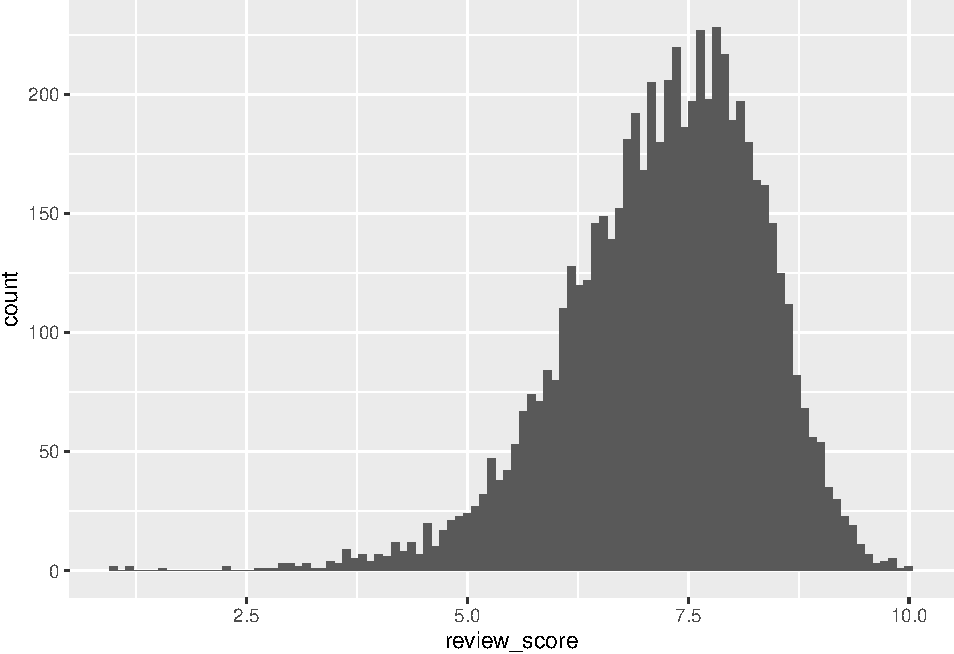
\includegraphics{1.3-data.cleaning_files/figure-latex/unnamed-chunk-1-1.pdf}

\begin{Shaded}
\begin{Highlighting}[]
 
\NormalTok{booking }\SpecialCharTok{\%\textgreater{}\%} 
  \FunctionTok{ggplot}\NormalTok{(}
    \FunctionTok{aes}\NormalTok{(price\_per\_night,review\_score)}
\NormalTok{  )}\SpecialCharTok{+}\FunctionTok{geom\_point}\NormalTok{()}
\CommentTok{\#\textgreater{} Warning: Removed 3817 rows containing missing values}
\CommentTok{\#\textgreater{} (geom\_point).}
\end{Highlighting}
\end{Shaded}

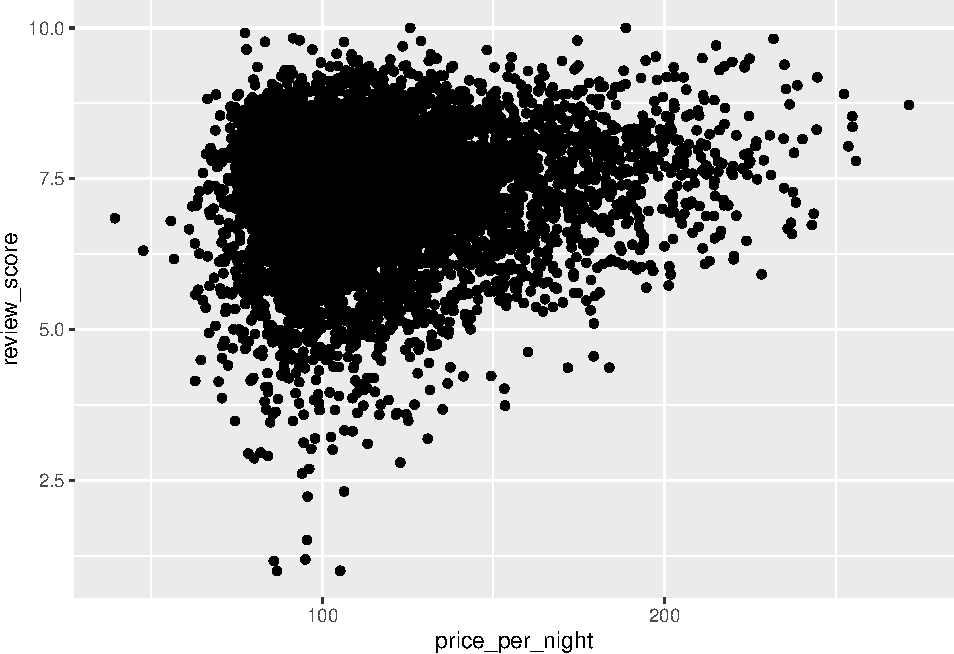
\includegraphics{1.3-data.cleaning_files/figure-latex/unnamed-chunk-1-2.pdf}

\begin{Shaded}
\begin{Highlighting}[]
 
\NormalTok{booking }\SpecialCharTok{\%\textgreater{}\%} 
  \FunctionTok{filter}\NormalTok{(room\_nights}\SpecialCharTok{\textgreater{}}\DecValTok{7}\NormalTok{, status}\SpecialCharTok{==}\StringTok{\textquotesingle{}stayed\textquotesingle{}}\NormalTok{) }\SpecialCharTok{\%\textgreater{}\%} 
  \FunctionTok{select}\NormalTok{(price\_per\_night,review\_score) }\SpecialCharTok{\%\textgreater{}\%} 
  \FunctionTok{ggplot}\NormalTok{(}
    \FunctionTok{aes}\NormalTok{(price\_per\_night,review\_score)}
\NormalTok{  )}\SpecialCharTok{+}\FunctionTok{geom\_point}\NormalTok{()}
\CommentTok{\#\textgreater{} Warning: Removed 41 rows containing missing values}
\CommentTok{\#\textgreater{} (geom\_point).}
\end{Highlighting}
\end{Shaded}

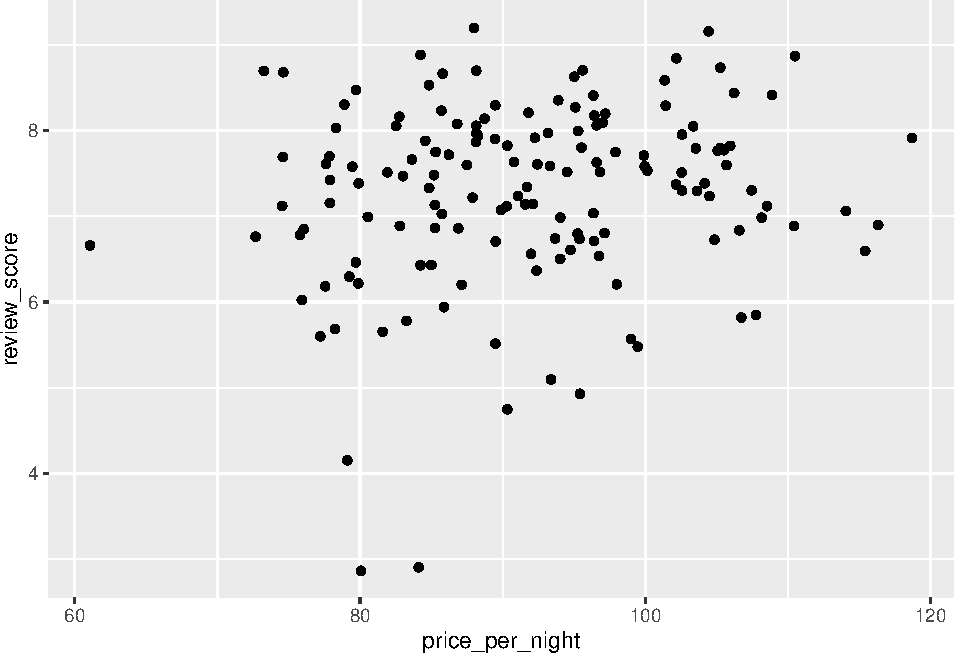
\includegraphics{1.3-data.cleaning_files/figure-latex/unnamed-chunk-1-3.pdf}

\begin{Shaded}
\begin{Highlighting}[]

\CommentTok{\#mutate}

\NormalTok{booking }\SpecialCharTok{\%\textgreater{}\%} 
  \FunctionTok{mutate}\NormalTok{(}\AttributeTok{centered\_mean=}\NormalTok{price\_per\_night}\SpecialCharTok{{-}}\FunctionTok{mean}\NormalTok{(price\_per\_night)) }\SpecialCharTok{\%\textgreater{}\%} 
  \FunctionTok{head}\NormalTok{(}\DecValTok{2}\NormalTok{)}
\CommentTok{\#\textgreater{} \# A tibble: 2 x 9}
\CommentTok{\#\textgreater{}   booker\_id          property\_id room\_nights price\_per\_night}
\CommentTok{\#\textgreater{}   \textless{}chr\textgreater{}                    \textless{}dbl\textgreater{}       \textless{}dbl\textgreater{}           \textless{}dbl\textgreater{}}
\CommentTok{\#\textgreater{} 1 215934017ba98c09f\textasciitilde{}        2668           4            91.5}
\CommentTok{\#\textgreater{} 2 7f590fd6d318248a4\textasciitilde{}        4656           5           107. }
\CommentTok{\#\textgreater{} \# ... with 5 more variables: checkin\_day \textless{}chr\textgreater{},}
\CommentTok{\#\textgreater{} \#   for\_business \textless{}lgl\textgreater{}, status \textless{}chr\textgreater{}, review\_score \textless{}dbl\textgreater{},}
\CommentTok{\#\textgreater{} \#   centered\_mean \textless{}dbl\textgreater{}}

\CommentTok{\# summarise: extracts the number of variables}

\NormalTok{booking }\SpecialCharTok{\%\textgreater{}\%} 
  \FunctionTok{summarise}\NormalTok{(}
    \FunctionTok{n}\NormalTok{()}
\NormalTok{    , }\AttributeTok{n\_miss=}\FunctionTok{sum}\NormalTok{(}\FunctionTok{is.na}\NormalTok{(review\_score))}
\NormalTok{    ,}\AttributeTok{mean\_score=}\FunctionTok{mean}\NormalTok{(review\_score,}\AttributeTok{na.rm=}\NormalTok{T))}
\CommentTok{\#\textgreater{} \# A tibble: 1 x 3}
\CommentTok{\#\textgreater{}   \textasciigrave{}n()\textasciigrave{} n\_miss mean\_score}
\CommentTok{\#\textgreater{}   \textless{}int\textgreater{}  \textless{}int\textgreater{}      \textless{}dbl\textgreater{}}
\CommentTok{\#\textgreater{} 1 10000   3817       7.22}

\NormalTok{booking }\SpecialCharTok{\%\textgreater{}\%} 
  \FunctionTok{summarise}\NormalTok{(}
     \FunctionTok{n}\NormalTok{()}
\NormalTok{    , }\AttributeTok{stayed\_booking=}\FunctionTok{sum}\NormalTok{(status}\SpecialCharTok{==}\StringTok{\textquotesingle{}stayed\textquotesingle{}}\NormalTok{)}
\NormalTok{    , }\AttributeTok{mean\_total=}\FunctionTok{mean}\NormalTok{(price\_per\_night}\SpecialCharTok{*}\NormalTok{room\_nights)                   }
                         
\NormalTok{  )}
\CommentTok{\#\textgreater{} \# A tibble: 1 x 3}
\CommentTok{\#\textgreater{}   \textasciigrave{}n()\textasciigrave{} stayed\_booking mean\_total}
\CommentTok{\#\textgreater{}   \textless{}int\textgreater{}          \textless{}int\textgreater{}      \textless{}dbl\textgreater{}}
\CommentTok{\#\textgreater{} 1 10000           7775       348.}
\CommentTok{\#group by}
\NormalTok{booking }\SpecialCharTok{\%\textgreater{}\%} 
  \FunctionTok{group\_by}\NormalTok{(}
\NormalTok{    for\_business}
\NormalTok{  ) }\SpecialCharTok{\%\textgreater{}\%} 
  \FunctionTok{summarise}\NormalTok{(}
  \AttributeTok{n=}\FunctionTok{n}\NormalTok{()}
\NormalTok{, }\AttributeTok{mean\_review=}\FunctionTok{mean}\NormalTok{(review\_score,}\AttributeTok{na.rm=}\NormalTok{T))}
\CommentTok{\#\textgreater{} \# A tibble: 2 x 3}
\CommentTok{\#\textgreater{}   for\_business     n mean\_review}
\CommentTok{\#\textgreater{}   \textless{}lgl\textgreater{}        \textless{}int\textgreater{}       \textless{}dbl\textgreater{}}
\CommentTok{\#\textgreater{} 1 FALSE         6285        7.50}
\CommentTok{\#\textgreater{} 2 TRUE          3715        6.85}

\NormalTok{mixed}\OtherTok{=}\NormalTok{booking }\SpecialCharTok{\%\textgreater{}\%} 
  \FunctionTok{full\_join}\NormalTok{(property) }\SpecialCharTok{\%\textgreater{}\%} 
  \FunctionTok{count}\NormalTok{(destination,checkin\_day) }\SpecialCharTok{\%\textgreater{}\%} 
  \FunctionTok{pivot\_wider}\NormalTok{(}
    \AttributeTok{names\_from =}\NormalTok{ checkin\_day,}\AttributeTok{values\_from =}\NormalTok{ n}
\NormalTok{  )}
\CommentTok{\#\textgreater{} Joining, by = "property\_id"}
\NormalTok{mixed }
\CommentTok{\#\textgreater{} \# A tibble: 3 x 8}
\CommentTok{\#\textgreater{}   destination   fri   mon   sat   sun   thu   tue   wed}
\CommentTok{\#\textgreater{}   \textless{}chr\textgreater{}       \textless{}int\textgreater{} \textless{}int\textgreater{} \textless{}int\textgreater{} \textless{}int\textgreater{} \textless{}int\textgreater{} \textless{}int\textgreater{} \textless{}int\textgreater{}}
\CommentTok{\#\textgreater{} 1 Amsterdam    1074   517   889   813   667   498   542}
\CommentTok{\#\textgreater{} 2 Brisbane      162   133   114   153   162   148   128}
\CommentTok{\#\textgreater{} 3 Tokyo         451   718   322   576   718   655   560}

\CommentTok{\# make a long data form}

\NormalTok{long}\OtherTok{=}\NormalTok{mixed}\SpecialCharTok{\%\textgreater{}\%}
  \FunctionTok{pivot\_longer}\NormalTok{(}\AttributeTok{cols =} \DecValTok{2}\SpecialCharTok{:}\DecValTok{8}\NormalTok{, }\AttributeTok{names\_to =} \StringTok{\textquotesingle{}day\textquotesingle{}}\NormalTok{,}\AttributeTok{values\_to =} \StringTok{\textquotesingle{}count\textquotesingle{}}\NormalTok{)}
\NormalTok{long}
\CommentTok{\#\textgreater{} \# A tibble: 21 x 3}
\CommentTok{\#\textgreater{}    destination day   count}
\CommentTok{\#\textgreater{}    \textless{}chr\textgreater{}       \textless{}chr\textgreater{} \textless{}int\textgreater{}}
\CommentTok{\#\textgreater{}  1 Amsterdam   fri    1074}
\CommentTok{\#\textgreater{}  2 Amsterdam   mon     517}
\CommentTok{\#\textgreater{}  3 Amsterdam   sat     889}
\CommentTok{\#\textgreater{}  4 Amsterdam   sun     813}
\CommentTok{\#\textgreater{}  5 Amsterdam   thu     667}
\CommentTok{\#\textgreater{}  6 Amsterdam   tue     498}
\CommentTok{\#\textgreater{}  7 Amsterdam   wed     542}
\CommentTok{\#\textgreater{}  8 Brisbane    fri     162}
\CommentTok{\#\textgreater{}  9 Brisbane    mon     133}
\CommentTok{\#\textgreater{} 10 Brisbane    sat     114}
\CommentTok{\#\textgreater{} \# ... with 11 more rows}

\CommentTok{\# make long data form}

\NormalTok{wide}\OtherTok{=}\NormalTok{ long }\SpecialCharTok{\%\textgreater{}\%} 
  \FunctionTok{pivot\_wider}\NormalTok{(}\AttributeTok{names\_from =} \StringTok{"day"}\NormalTok{, }\AttributeTok{values\_from =} \StringTok{"count"}\NormalTok{)}
\NormalTok{wide}
\CommentTok{\#\textgreater{} \# A tibble: 3 x 8}
\CommentTok{\#\textgreater{}   destination   fri   mon   sat   sun   thu   tue   wed}
\CommentTok{\#\textgreater{}   \textless{}chr\textgreater{}       \textless{}int\textgreater{} \textless{}int\textgreater{} \textless{}int\textgreater{} \textless{}int\textgreater{} \textless{}int\textgreater{} \textless{}int\textgreater{} \textless{}int\textgreater{}}
\CommentTok{\#\textgreater{} 1 Amsterdam    1074   517   889   813   667   498   542}
\CommentTok{\#\textgreater{} 2 Brisbane      162   133   114   153   162   148   128}
\CommentTok{\#\textgreater{} 3 Tokyo         451   718   322   576   718   655   560}


\CommentTok{\# Boxplot with ggplot2}
\NormalTok{booking }\SpecialCharTok{\%\textgreater{}\%} 
  \FunctionTok{ggplot}\NormalTok{(}
    \FunctionTok{aes}\NormalTok{(}
\NormalTok{      review\_score,for\_business}
\NormalTok{    )}
\NormalTok{  )}\SpecialCharTok{+}\FunctionTok{geom\_boxplot}\NormalTok{()}
\CommentTok{\#\textgreater{} Warning: Removed 3817 rows containing non{-}finite values}
\CommentTok{\#\textgreater{} (stat\_boxplot).}
\end{Highlighting}
\end{Shaded}

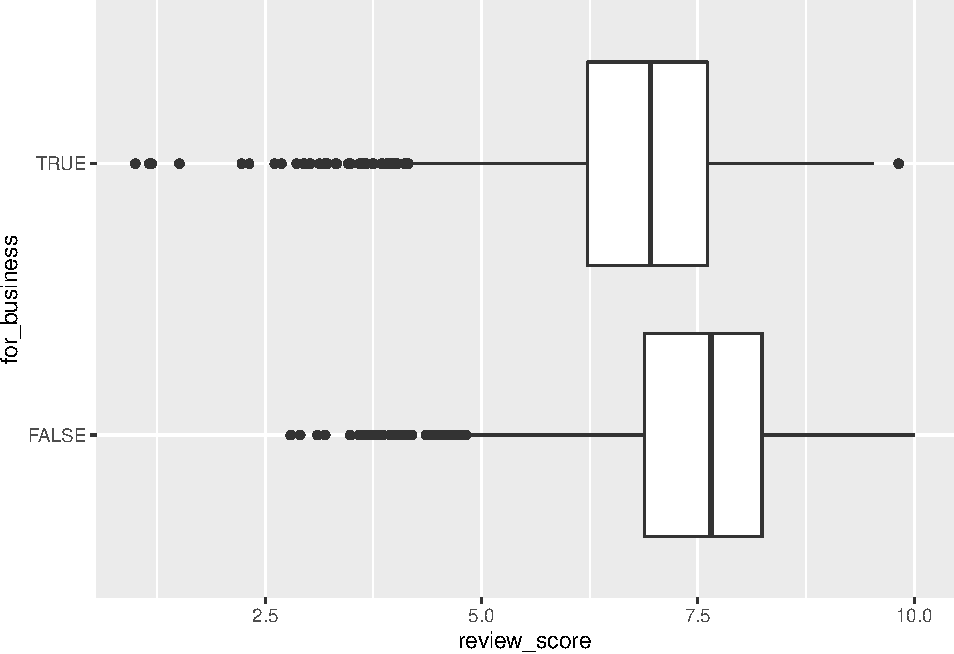
\includegraphics{1.3-data.cleaning_files/figure-latex/unnamed-chunk-1-4.pdf}

\begin{Shaded}
\begin{Highlighting}[]
    
\CommentTok{\# hash the property id}
\CommentTok{\# we need to know map()function to do this. map(x,\textasciitilde{}.), where x = object and \textasciitilde{}. is a function which goes through each vector}
\FunctionTok{library}\NormalTok{(digest)}

\NormalTok{property }\SpecialCharTok{\%\textgreater{}\%} 
  \FunctionTok{mutate}\NormalTok{(}\AttributeTok{property\_id=}\FunctionTok{map\_chr}\NormalTok{(property\_id,digest))}
\CommentTok{\#\textgreater{} \# A tibble: 4,178 x 5}
\CommentTok{\#\textgreater{}    property\_id destination property\_type nr\_rooms facilities}
\CommentTok{\#\textgreater{}    \textless{}chr\textgreater{}       \textless{}chr\textgreater{}       \textless{}chr\textgreater{}            \textless{}dbl\textgreater{} \textless{}chr\textgreater{}     }
\CommentTok{\#\textgreater{}  1 c5fe5a36c3\textasciitilde{} Brisbane    Hotel               32 airport s\textasciitilde{}}
\CommentTok{\#\textgreater{}  2 6abfc65c14\textasciitilde{} Brisbane    Hotel               39 on{-}site r\textasciitilde{}}
\CommentTok{\#\textgreater{}  3 8740143b90\textasciitilde{} Brisbane    Apartment            9 laundry   }
\CommentTok{\#\textgreater{}  4 e30b95c1ec\textasciitilde{} Brisbane    Apartment            9 kitchen,l\textasciitilde{}}
\CommentTok{\#\textgreater{}  5 ab19240af8\textasciitilde{} Brisbane    Apartment            4 parking,k\textasciitilde{}}
\CommentTok{\#\textgreater{}  6 b2efd881c3\textasciitilde{} Brisbane    Apartment            5 kitchen,p\textasciitilde{}}
\CommentTok{\#\textgreater{}  7 d49c23b12c\textasciitilde{} Brisbane    Hotel               22 airport s\textasciitilde{}}
\CommentTok{\#\textgreater{}  8 1fd9f14595\textasciitilde{} Brisbane    Hotel               20 breakfast\textasciitilde{}}
\CommentTok{\#\textgreater{}  9 7319c32a43\textasciitilde{} Brisbane    Apartment            5 free wifi\textasciitilde{}}
\CommentTok{\#\textgreater{} 10 a38cc66d5f\textasciitilde{} Brisbane    Apartment           11 free wifi\textasciitilde{}}
\CommentTok{\#\textgreater{} \# ... with 4,168 more rows}

\CommentTok{\# list in data frame}
\CommentTok{\# If we have a column with multiple strings, we can split it in to vectors using strsplit()}


\NormalTok{property }\SpecialCharTok{\%\textgreater{}\%} 
  \FunctionTok{mutate}\NormalTok{(}\AttributeTok{facilities=}\FunctionTok{strsplit}\NormalTok{(facilities,}\StringTok{","}\NormalTok{))}
\CommentTok{\#\textgreater{} \# A tibble: 4,178 x 5}
\CommentTok{\#\textgreater{}    property\_id destination property\_type nr\_rooms facilities}
\CommentTok{\#\textgreater{}          \textless{}dbl\textgreater{} \textless{}chr\textgreater{}       \textless{}chr\textgreater{}            \textless{}dbl\textgreater{} \textless{}list\textgreater{}    }
\CommentTok{\#\textgreater{}  1        2668 Brisbane    Hotel               32 \textless{}chr [6]\textgreater{} }
\CommentTok{\#\textgreater{}  2        4656 Brisbane    Hotel               39 \textless{}chr [7]\textgreater{} }
\CommentTok{\#\textgreater{}  3        4563 Brisbane    Apartment            9 \textless{}chr [1]\textgreater{} }
\CommentTok{\#\textgreater{}  4        4088 Brisbane    Apartment            9 \textless{}chr [3]\textgreater{} }
\CommentTok{\#\textgreater{}  5        2188 Brisbane    Apartment            4 \textless{}chr [5]\textgreater{} }
\CommentTok{\#\textgreater{}  6        4171 Brisbane    Apartment            5 \textless{}chr [6]\textgreater{} }
\CommentTok{\#\textgreater{}  7        2907 Brisbane    Hotel               22 \textless{}chr [8]\textgreater{} }
\CommentTok{\#\textgreater{}  8        5141 Brisbane    Hotel               20 \textless{}chr [8]\textgreater{} }
\CommentTok{\#\textgreater{}  9        1696 Brisbane    Apartment            5 \textless{}chr [6]\textgreater{} }
\CommentTok{\#\textgreater{} 10        1901 Brisbane    Apartment           11 \textless{}chr [8]\textgreater{} }
\CommentTok{\#\textgreater{} \# ... with 4,168 more rows}
\NormalTok{property}\SpecialCharTok{$}\NormalTok{facilities[}\DecValTok{1}\NormalTok{]}
\CommentTok{\#\textgreater{} [1] "airport shuttle,free wifi,garden,breakfast,pool,on{-}site restaurant"}

\CommentTok{\# add a column with the number of facilities}

\NormalTok{property }\SpecialCharTok{\%\textgreater{}\%}
  \FunctionTok{mutate}\NormalTok{(}\AttributeTok{facilities=}\FunctionTok{strsplit}\NormalTok{(facilities,}\StringTok{","}\NormalTok{)) }\SpecialCharTok{\%\textgreater{}\%} 
  \FunctionTok{mutate}\NormalTok{(}\AttributeTok{n\_facility=}\FunctionTok{map\_int}\NormalTok{(facilities,length))}
\CommentTok{\#\textgreater{} \# A tibble: 4,178 x 6}
\CommentTok{\#\textgreater{}    property\_id destination property\_type nr\_rooms facilities}
\CommentTok{\#\textgreater{}          \textless{}dbl\textgreater{} \textless{}chr\textgreater{}       \textless{}chr\textgreater{}            \textless{}dbl\textgreater{} \textless{}list\textgreater{}    }
\CommentTok{\#\textgreater{}  1        2668 Brisbane    Hotel               32 \textless{}chr [6]\textgreater{} }
\CommentTok{\#\textgreater{}  2        4656 Brisbane    Hotel               39 \textless{}chr [7]\textgreater{} }
\CommentTok{\#\textgreater{}  3        4563 Brisbane    Apartment            9 \textless{}chr [1]\textgreater{} }
\CommentTok{\#\textgreater{}  4        4088 Brisbane    Apartment            9 \textless{}chr [3]\textgreater{} }
\CommentTok{\#\textgreater{}  5        2188 Brisbane    Apartment            4 \textless{}chr [5]\textgreater{} }
\CommentTok{\#\textgreater{}  6        4171 Brisbane    Apartment            5 \textless{}chr [6]\textgreater{} }
\CommentTok{\#\textgreater{}  7        2907 Brisbane    Hotel               22 \textless{}chr [8]\textgreater{} }
\CommentTok{\#\textgreater{}  8        5141 Brisbane    Hotel               20 \textless{}chr [8]\textgreater{} }
\CommentTok{\#\textgreater{}  9        1696 Brisbane    Apartment            5 \textless{}chr [6]\textgreater{} }
\CommentTok{\#\textgreater{} 10        1901 Brisbane    Apartment           11 \textless{}chr [8]\textgreater{} }
\CommentTok{\#\textgreater{} \# ... with 4,168 more rows, and 1 more variable:}
\CommentTok{\#\textgreater{} \#   n\_facility \textless{}int\textgreater{}}
\end{Highlighting}
\end{Shaded}


\end{document}
